%!TEX root = hw_7.tex
\subsection*{Team Contributions}
We collaborated back and forth and between pull requests we made sure everything functioned well across both our machines. 
This led to not having a strict boundary between components implemented by each of us. That being said the core components we worked on are divided
in a more divided way are as follows.
Horacio Moreno Monta\~nes: \lstinline{initial_conditions, multigrid, pressure_solver, output, plotting}
Neil MacLachlan: \lstinline{physics, integrator, viscous_solver, boundary_conditions, grid, spack}
\section*{Problem 1: 2D Navier--Stokes Solver for the Taylor--Green Vortex}

In this assignment, you will extend your pressure projection solver to a full incompressible Navier--Stokes solver in two dimensions. You will simulate the decay of the \emph{Taylor--Green vortex}, a canonical benchmark for transitional and decaying turbulence.

\subsection*{Governing Equations}

We consider the two-dimensional Navier--Stokes equations in the incompressible limit and non-dimensional form:
\begin{align}
  \frac{\partial u}{\partial x} + \frac{\partial v}{\partial y} &= 0, \label{eq:continuity} \\
  \frac{\partial u}{\partial t} + \frac{\partial uu}{\partial x} + \frac{\partial uv}{\partial y} &= -\frac{\partial p}{\partial x} + \frac{1}{\mathrm{Re}} \left( \frac{\partial^2 u}{\partial x^2} + \frac{\partial^2 u}{\partial y^2} \right), \label{eq:umom} \\
  \frac{\partial v}{\partial t} + \frac{\partial uv}{\partial x} + \frac{\partial vv}{\partial y} &= -\frac{\partial p}{\partial y} + \frac{1}{\mathrm{Re}} \left( \frac{\partial^2 v}{\partial x^2} + \frac{\partial^2 v}{\partial y^2} \right), \label{eq:vmom}
\end{align}
where $\mathrm{Re}$ is the Reynolds number.

\subsection*{Domain and Grid}

\begin{itemize}
  \item Domain: $[0, 2\pi]^2$
  \item Uniform (staggered) grid: $64 \times 64$
  \item Periodic boundary conditions in all directions
\end{itemize}

\subsection*{Initial Condition (Taylor--Green Vortex)}

\begin{align}
  u(x,y; t=0) &= \sin(x)\cos(y), \label{eq:ic_u} \\
  v(x,y; t=0) &= -\cos(x)\sin(y). \label{eq:ic_v}
\end{align}

\subsection*{Numerical Method}

Use a \emph{fractional step (projection) method} with second-order spatial discretization and Crank--Nicolson time integration for viscous terms. Use the Thomas algorithm for solving the viscous terms implicitly (tridiagonal solver in $x$- and $y$-directions using ADI splitting). Use the Sherman--Morrison correction for periodic boundary conditions. Use multigrid for the pressure Poisson equation.

\subsubsection*{Staggered Variable Arrangement}

For cell $(i,j)$, store velocity $u$ at the barycenter of the left face ($u_{i-\frac{1}{2},j}$), $v$ at the barycenter of the bottom face ($v_{i,j-\frac{1}{2}}$), and pressure $p$ at the cell center ($p_{i,j}$). The solenoidal constraint is discretized as:
\begin{equation}
  \nabla \cdot \mathbf{u}\big|_{i,j} \approx \frac{u_{i+\frac{1}{2},j} - u_{i-\frac{1}{2},j}}{\Delta x} + \frac{v_{i,j+\frac{1}{2}} - v_{i,j-\frac{1}{2}}}{\Delta y}. \label{eq:div}
\end{equation}

\subsubsection*{Spatial Discretization (u-momentum)}

Convective term in $x$:
\begin{equation}
  \left.\frac{\partial uu}{\partial x}\right|_{i-\frac{1}{2},j} \approx \frac{u_{i,j}^2 - u_{i-1,j}^2}{\Delta x} \label{eq:conv_x}
\end{equation}

Convective term in $y$:
\begin{equation}
  \left.\frac{\partial uv}{\partial y}\right|_{i-\frac{1}{2},j} \approx \frac{u_{i-\frac{1}{2},j+\frac{1}{2}} v_{i-\frac{1}{2},j+\frac{1}{2}} - u_{i-\frac{1}{2},j-\frac{1}{2}} v_{i-\frac{1}{2},j-\frac{1}{2}}}{\Delta y} \label{eq:conv_y}
\end{equation}

Viscous term in $x$:
\begin{equation}
  \left.\frac{\partial^2 u}{\partial x^2}\right|_{i-\frac{1}{2},j} \approx \frac{u_{i+\frac{1}{2},j} - 2u_{i-\frac{1}{2},j} + u_{i-\frac{3}{2},j}}{\Delta x^2} \label{eq:visc_x}
\end{equation}

Viscous term in $y$:
\begin{equation}
  \left.\frac{\partial^2 u}{\partial y^2}\right|_{i-\frac{1}{2},j} \approx \frac{u_{i-\frac{1}{2},j+1} - 2u_{i-\frac{1}{2},j} + u_{i-\frac{1}{2},j-1}}{\Delta y^2} \label{eq:visc_y}
\end{equation}

Pressure term in $x$:
\begin{equation}
  \left.\frac{\partial p}{\partial x}\right|_{i-\frac{1}{2},j} \approx \frac{p_{i,j} - p_{i-1,j}}{\Delta x} \label{eq:pres_x}
\end{equation}

Additional interpolations:
\begin{align}
  u_{i,j} &= \frac{1}{2}\left(u_{i-\frac{1}{2},j} + u_{i+\frac{1}{2},j}\right), \label{eq:u_interp} \\
  u_{i-\frac{1}{2},j-\frac{1}{2}} &= \frac{1}{2}\left(u_{i-\frac{1}{2},j} + u_{i-\frac{1}{2},j-1}\right), \label{eq:u_half_interp} \\
  v_{i-\frac{1}{2},j-\frac{1}{2}} &= \frac{1}{2}\left(v_{i,j-\frac{1}{2}} + v_{i-1,j-\frac{1}{2}}\right). \label{eq:v_half_interp}
\end{align}

\textbf{Observations:}
\begin{enumerate}
  \item All approximations are centered in space and formally second-order accurate.
  \item When coding, use $u(i,j) = u_{i-\frac{1}{2},j}$, $v(i,j) = v_{i,j-\frac{1}{2}}$, and $p(i,j) = p_{i,j}$.
  \item The $v$-momentum equation can be obtained readily from the proposed discretization of the $u$-momentum equation.
\end{enumerate}

\subsubsection*{Temporal Discretization -- Fractional Step Method}

Following Kim and Moin (1985), the method combines Adams--Bashforth for convective terms with Crank--Nicolson for viscous terms, and a projection step for pressure coupling.

\textbf{Step 1.} Advance momentum without pressure. Let $H$ denote the convective term:
\begin{equation}
  \frac{\mathbf{u}^\star_{i,j} - \mathbf{u}^n_{i,j}}{\Delta t} = \frac{3}{2}H^n_{i,j} - \frac{1}{2}H^{n-1}_{i,j} + \frac{1}{2\,\mathrm{Re}}\left(\frac{\delta^2}{\delta x^2} + \frac{\delta^2}{\delta y^2}\right)\left(\mathbf{u}^\star_{i,j} + \mathbf{u}^n_{i,j}\right). \label{eq:step1}
\end{equation}

Using approximate factorization (ADI splitting), this becomes two tridiagonal solves:
\begin{align}
  \left(1 - \frac{\Delta t}{2}\frac{1}{\mathrm{Re}}\frac{\delta^2}{\delta x^2}\right)\Delta \mathbf{u}^{\star\star}_{i,j} &= \frac{\Delta t}{2}\left(3H^n_{i,j} - H^{n-1}_{i,j}\right) + \frac{\Delta t}{\mathrm{Re}}\left(\frac{\delta^2}{\delta x^2} + \frac{\delta^2}{\delta y^2}\right)\mathbf{u}^n_{i,j}, \label{eq:adi_x} \\
  \left(1 - \frac{\Delta t}{2}\frac{1}{\mathrm{Re}}\frac{\delta^2}{\delta y^2}\right)\Delta \mathbf{u}^\star_{i,j} &= \Delta \mathbf{u}^{\star\star}_{i,j}, \label{eq:adi_y}
\end{align}
followed by the velocity update $\mathbf{u}^\star_{i,j} = \mathbf{u}^n_{i,j} + \Delta \mathbf{u}^\star_{i,j}$.

\textbf{Step 2.} Solve the pressure Poisson equation:
\begin{equation}
  \nabla \cdot \left(\nabla p^{n+1}\right)_{i,j} = \frac{1}{\Delta t}\nabla \cdot \mathbf{u}^\star\big|_{i,j}. \label{eq:ppe}
\end{equation}

\emph{Crucial observation:} The Laplacian in the pressure Poisson equation must be discretized exactly using the gradient and divergence operators from Steps 2 and 3.

\textbf{Step 3.} Correct the velocity:
\begin{equation}
  \mathbf{u}^{n+1}_{i,j} = \mathbf{u}^\star_{i,j} - \Delta t\,\nabla p^{n+1}\big|_{i,j}. \label{eq:correction}
\end{equation}

\subsubsection*{Time Stepping}

Choose $\Delta t$ such that:
\[
  \mathrm{CFL} = \frac{u_{\max}\Delta t}{\Delta x} \lesssim 0.5
\]
Simulate until $t = 10$.

\subsection*{Questions}

\subsubsection*{(a) Numerical Method Description}

% TODO: Provide a brief description of your numerical method, including:
% - Discretization of convective and diffusive terms
% - Structure of the Helmholtz solver
% - Linear solvers used

In this numerical method, we use both a cell-center grid for pressure $p$ and a cell-face grid for the velocities $u,v$. Therefore we approximate the convective terms according to Eqs. \eqref{eq:conv_x} \& \eqref{eq:conv_y} and the viscous diffusive terms according to Eqs. \eqref{eq:visc_x} \& \eqref{eq:visc_y}.

The time integration treats convection explicitly and uses a Crank Nicolson average for the diffusive term, therefore we have implicit diffusion, as shown in Eqs. \eqref{eq:adi_x} \& \eqref{eq:adi_y}. The explicit terms are computed directly as $\mathbf{rhs}$. Then the intermediate velocity $\mathbf{u}^\star$ is computed by solving the system 

\begin{equation}
  \left ( 1 - \frac{\Delta t}{2 \text{Re}} \nabla^2 \right ) \mathbf{u}^\star = \mathbf{rhs}.
\end{equation}

To do this linear solve, since we want to be able to run this in parallel systems we use a red-black Gauss-Seidel scheme. In such a scheme, the domain is split into black and red cells in a checkerboard pattern. Notice that all red cells depend only on black cells to compute the Laplacian and similarly all black cells depend only on the red cells. Therefore, in each iteration we do a red cell sweep followed by a black cell sweep, where only the red and black cells are updated respectively. With an access pattern like this, we ensure that parallel execution of kernels does not affect the result of the computation. The iterations are repeated, reapplying boundary conditions, until we achieve a desired tolerance or reach a maximum number of iterations. Using this Crank-Nicolson scheme ensures second-order accuracy in time and unconditional stability with respect to the viscous CFL constraint. 






\subsubsection*{(b) Incompressibility Verification}

% TODO: Plot either the max or L2 norm of divergence vs time

We plotted the root mean squared to make analysis independent of grid size for use in mesh refinement studies in the future.
This is the same the L2 norm variant suggested in previous homeworks. Our iterative solvers both use a tolerance of \lstinline{1e-8},
we thus expect the divergence to be of a similar order. We found that for CFL constraint values we chose and the Reynolds numbers we used
that the divergence was well below this. This may reflect the fact that the iterative methods can overshoot their tolerances. Interestingly in one 
case we saw a late rise in the divergence still well below the tolerance. We do not as yet have an explanation for this although 
since it is below tolerance it seems unlikely to be problematic. It may relate to the convergence of the red black scheme for the viscous term.
Lastly, note the initial value of the divergence is higher, but drops off. This is because we didn't initialize the pressure field with the same
analytical form as the velocities. This transient quickly vanishes.

\begin{figure}[htbp]
  \centering
  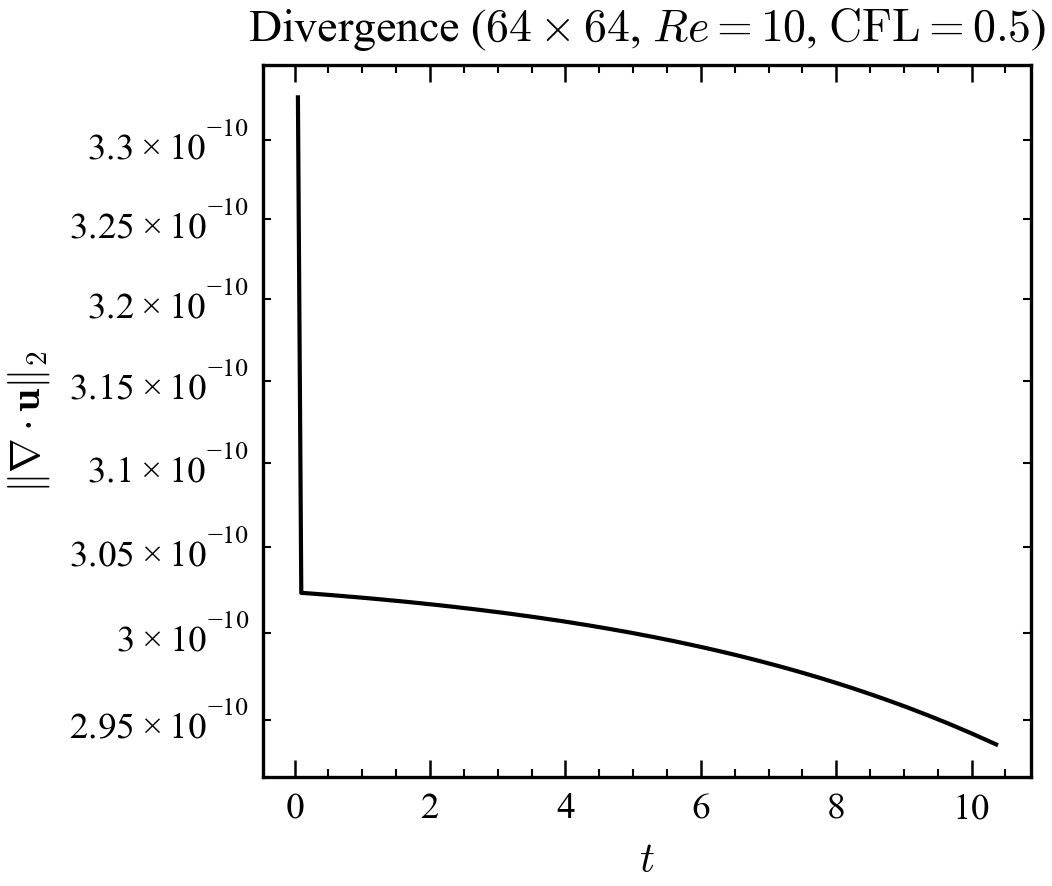
\includegraphics[width=0.32\textwidth]{images/divergence_re10_cfl0.5.png}
  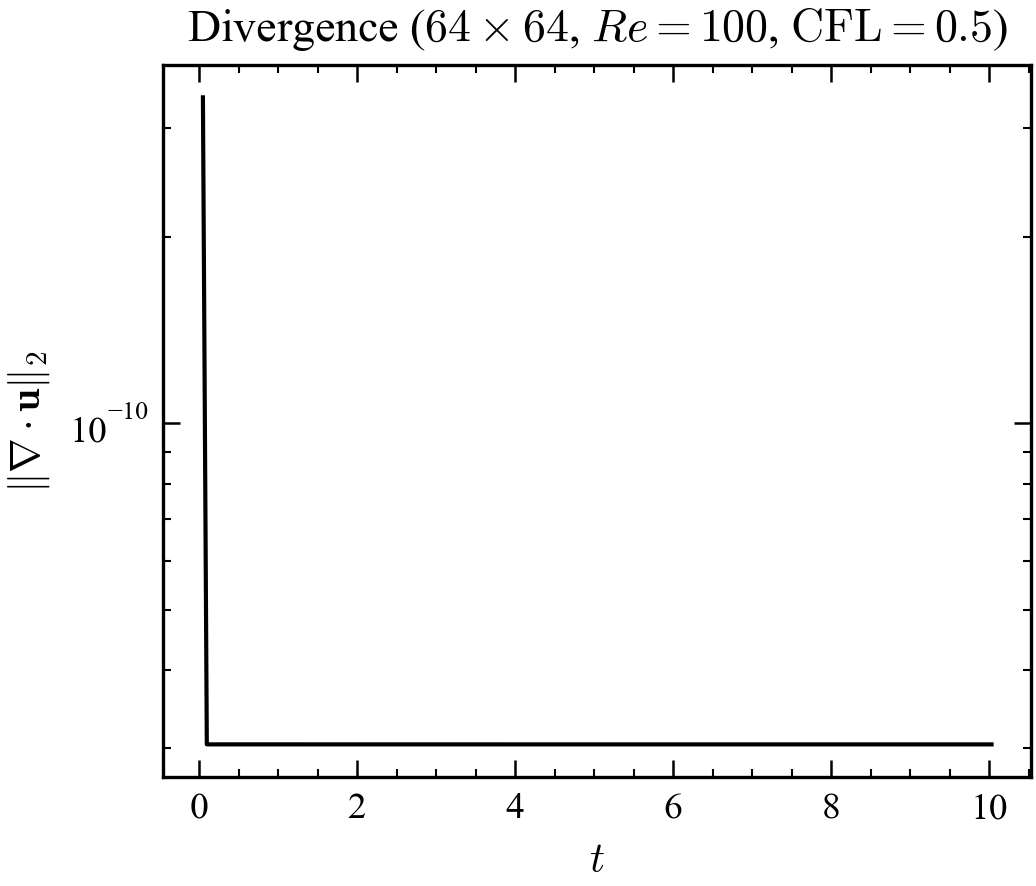
\includegraphics[width=0.32\textwidth]{images/divergence_re100_cfl0.5.png}
  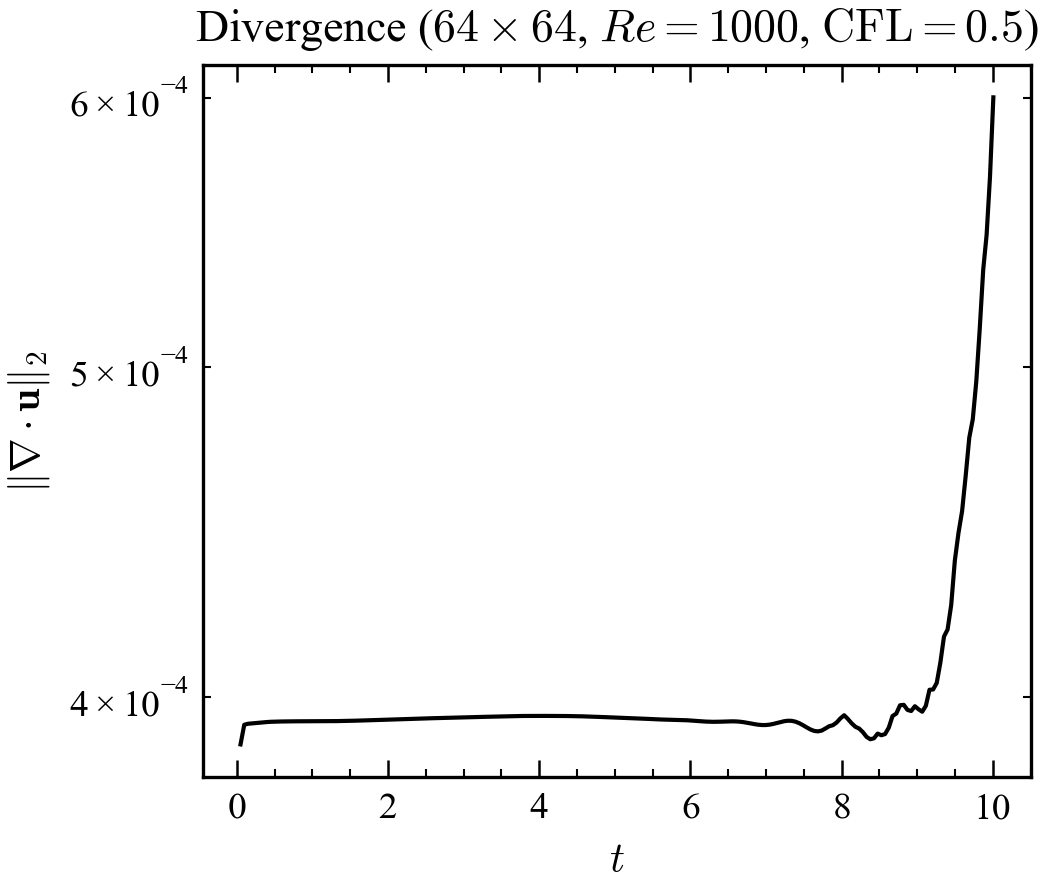
\includegraphics[width=0.32\textwidth]{images/divergence_re1000_cfl0.5.png}
  \caption{Incompressibility verification: $\ell^2$-norm of the discrete divergence $\|\nabla\cdot\mathbf{u}\|_2$ vs.\ time on a $64\times64$ grid, $\mathrm{CFL} = 0.5$, for $\mathrm{Re} = 10$, $100$, and $1000$ (left to right).}
  \label{fig:divergence}
\end{figure}


\subsubsection*{(c) Kinetic Energy}

% TODO: Compute and plot kinetic energy E(t) = 1/2 int |u|^2 dV
% Compare with expected decay behavior (analytic solution from HW1)

We define the kinetic energy of the fluid $E(t)$ by 

\begin{equation}
  E(t) = \frac{1}{2} \int |\mathbf{u}|^2 \dd V \approx \frac{1}{2} \sum_i |u_i|^2 \Delta x \Delta y.
\end{equation}

Figure \ref{fig:kinetic_energy} shows the decay of kinetic energy of the computed solution against the analytical decay rate. We can see that for larger Re values, the exponent is smaller and thus the decay is slower (almost linear) while for $\text{Re}=10$ we see a faster exponential decay. Moreover, we see that for all plots, the kinetic energy from the simulation agrees almost exactly with the exact value. 



\begin{figure}[htbp]
  \centering
  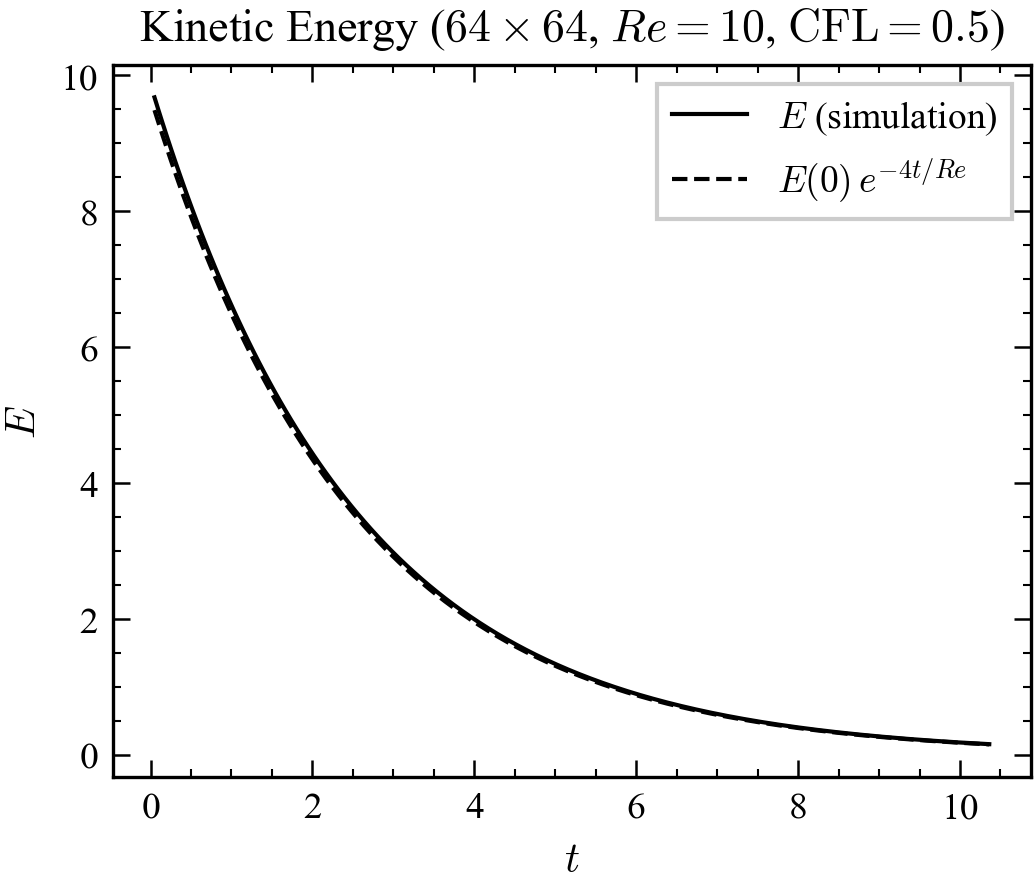
\includegraphics[width=0.32\textwidth]{images/kinetic_energy_re10_cfl0.5.png}
  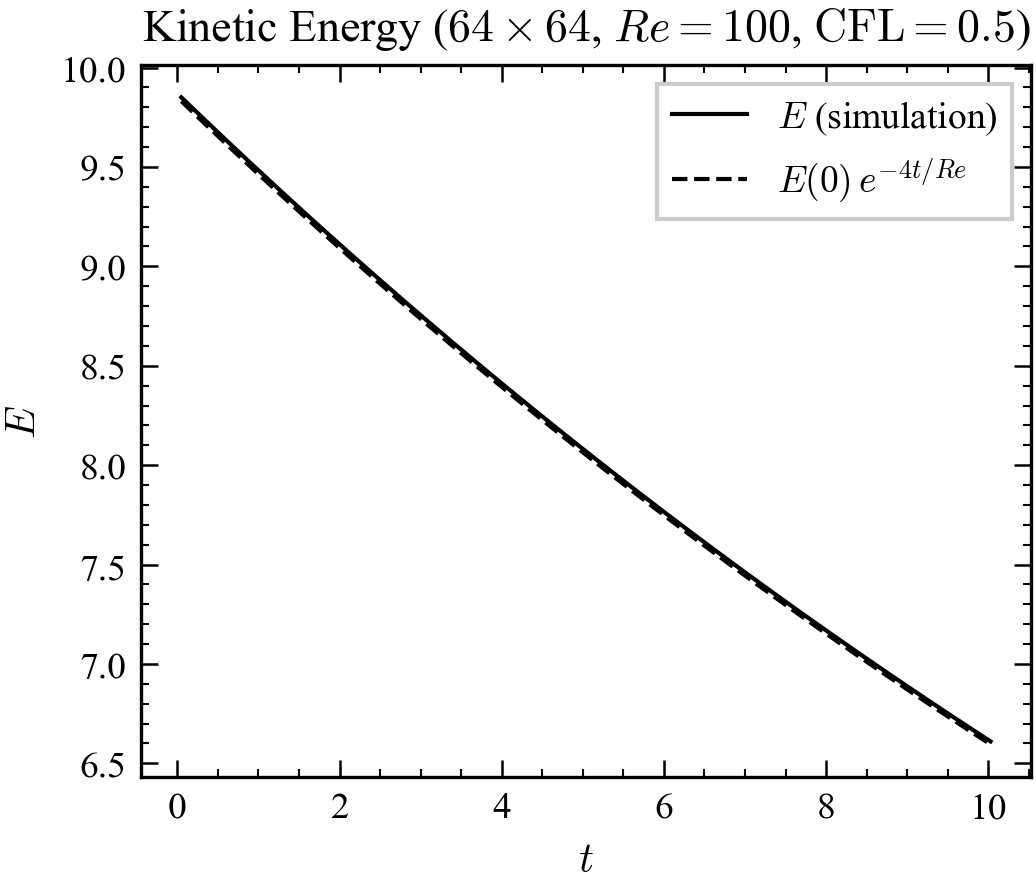
\includegraphics[width=0.32\textwidth]{images/kinetic_energy_re100_cfl0.5.png}
  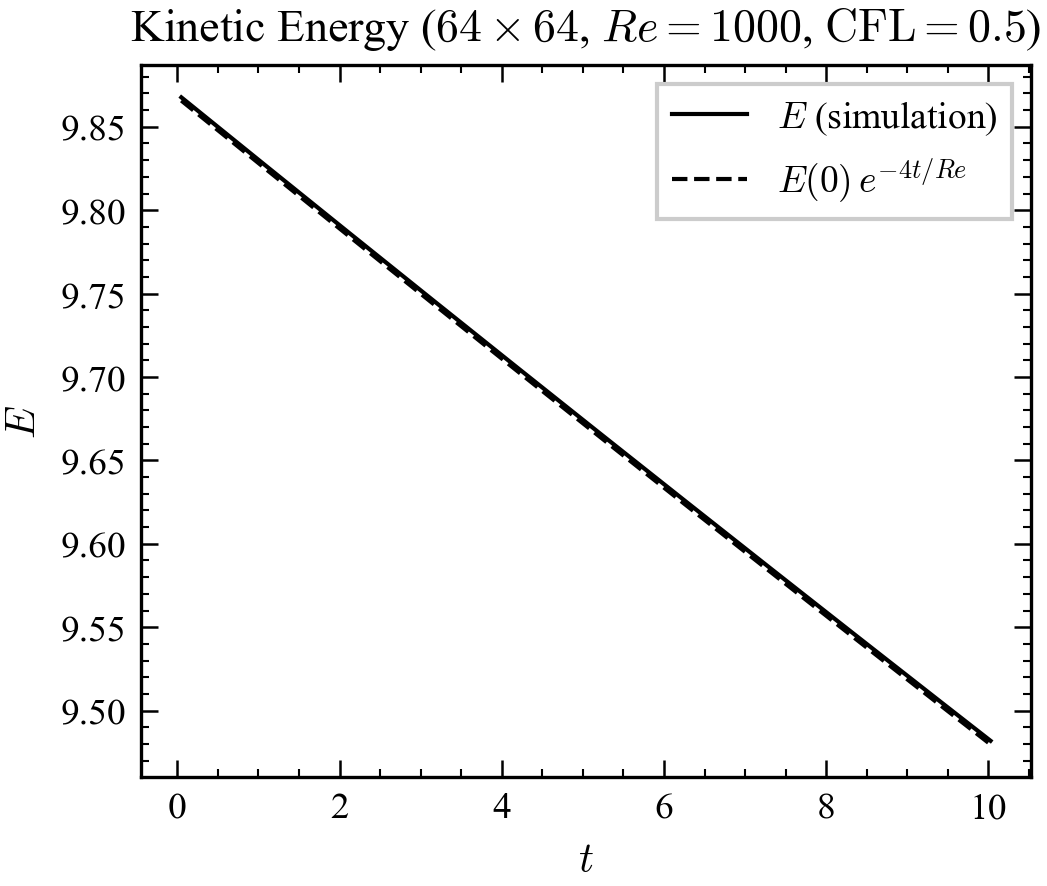
\includegraphics[width=0.32\textwidth]{images/kinetic_energy_re1000_cfl0.5.png}
  \caption{Kinetic energy decay $E(t) = \frac{1}{2}\int|\mathbf{u}|^2\,\mathrm{d}V$ for the Taylor--Green vortex on a $64\times64$ grid, $\mathrm{CFL} = 0.5$, for $\mathrm{Re} = 10$, $100$, and $1000$ (left to right). Dashed lines show the analytical decay $E_0\,e^{-4t/\mathrm{Re}}$.}
  \label{fig:kinetic_energy}
\end{figure}


\subsubsection*{(d) Flow Visualization}

\begin{figure}[htbp]
  \centering
  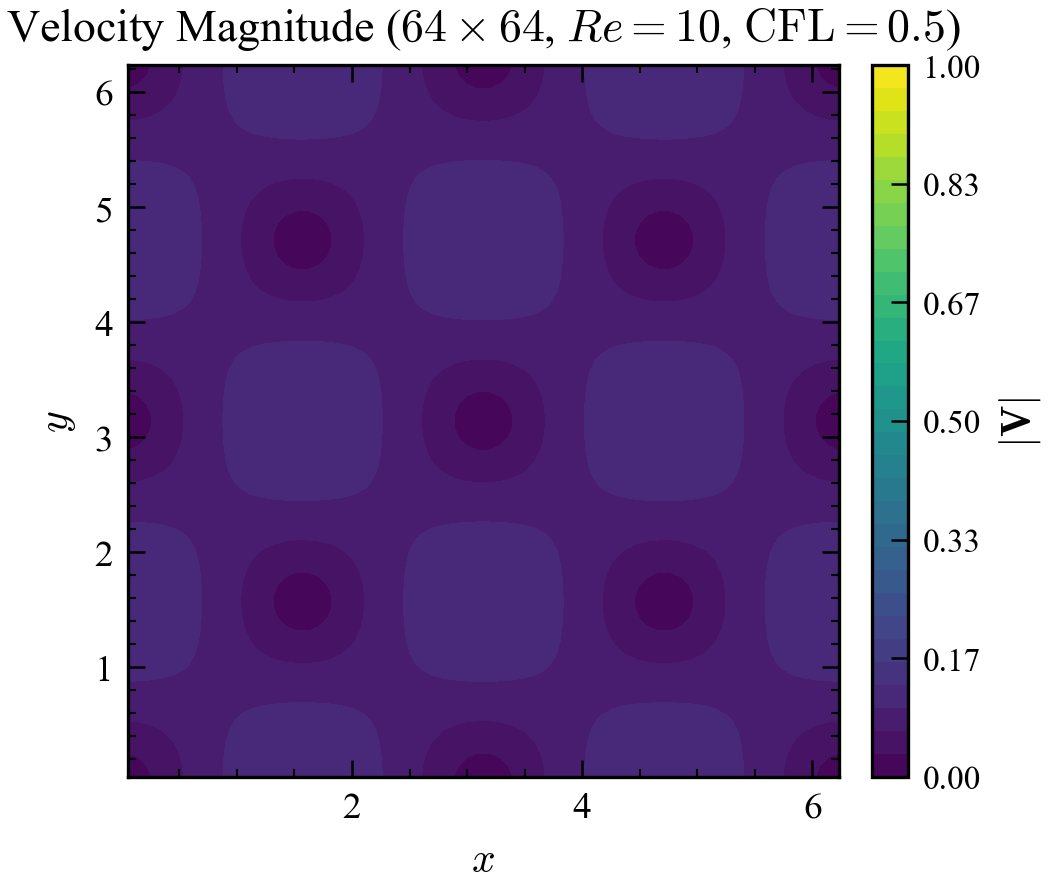
\includegraphics[width=0.32\textwidth]{images/velocity_magnitude_re10_cfl0.5.png}
  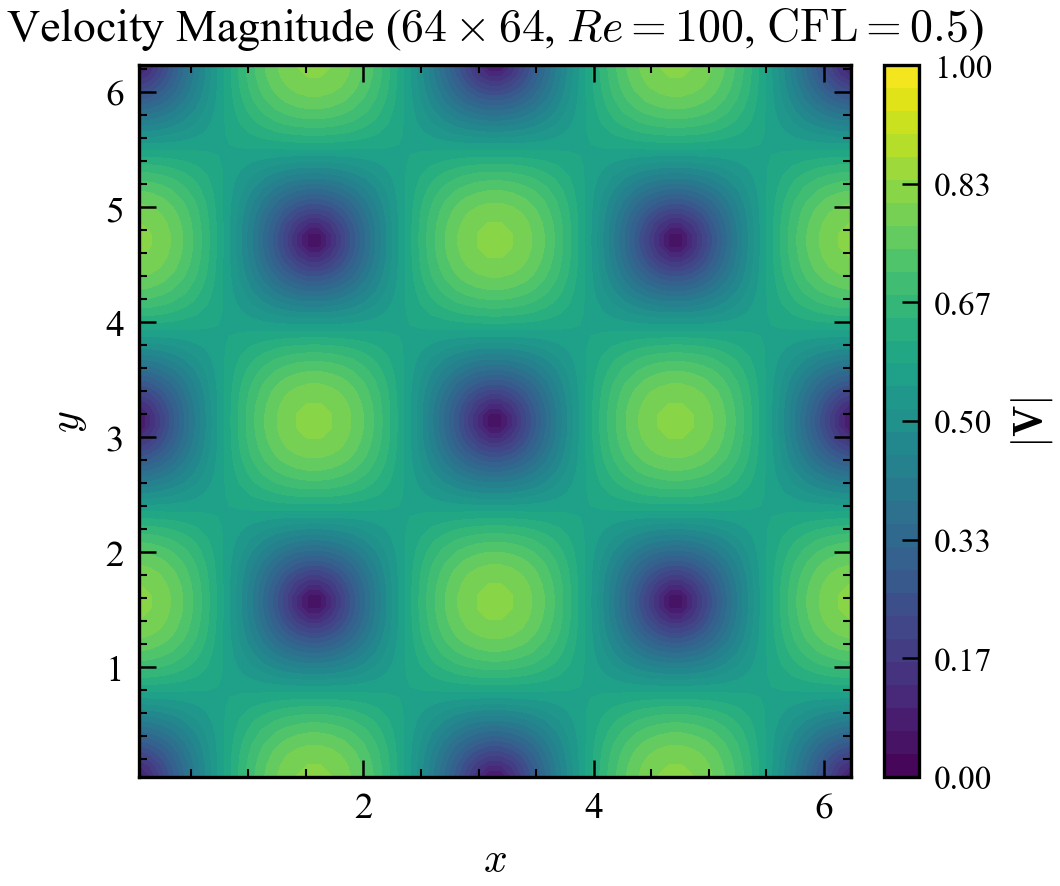
\includegraphics[width=0.32\textwidth]{images/velocity_magnitude_re100_cfl0.5.png}
  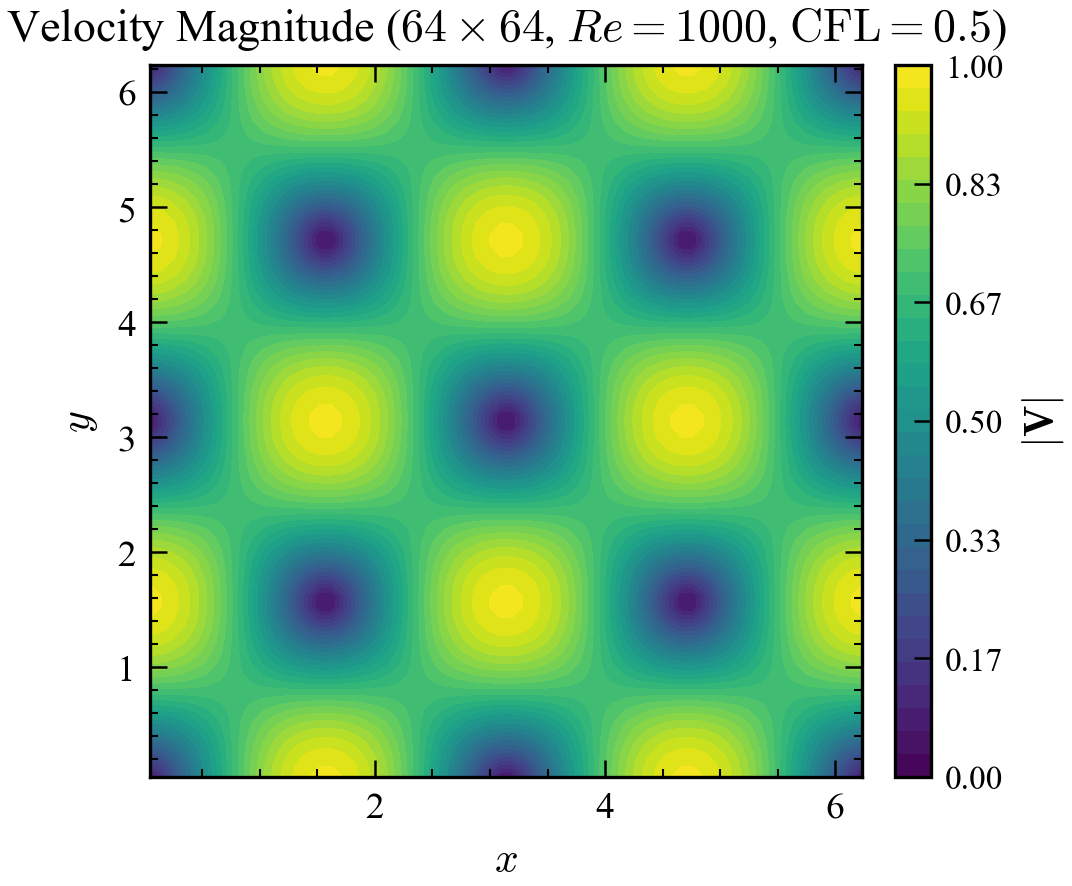
\includegraphics[width=0.32\textwidth]{images/velocity_magnitude_re1000_cfl0.5.png}
  \caption{Velocity magnitude contours $|\mathbf{u}| = \sqrt{u^2+v^2}$ at $t=10$ on a $64\times64$ grid, $\mathrm{CFL} = 0.5$, for $\mathrm{Re} = 10$, $100$, and $1000$ (left to right). Higher Re retains more vortex structure; lower Re shows stronger viscous dissipation.}
  \label{fig:velocity_magnitude}
\end{figure}

\begin{figure}[htbp]
  \centering
  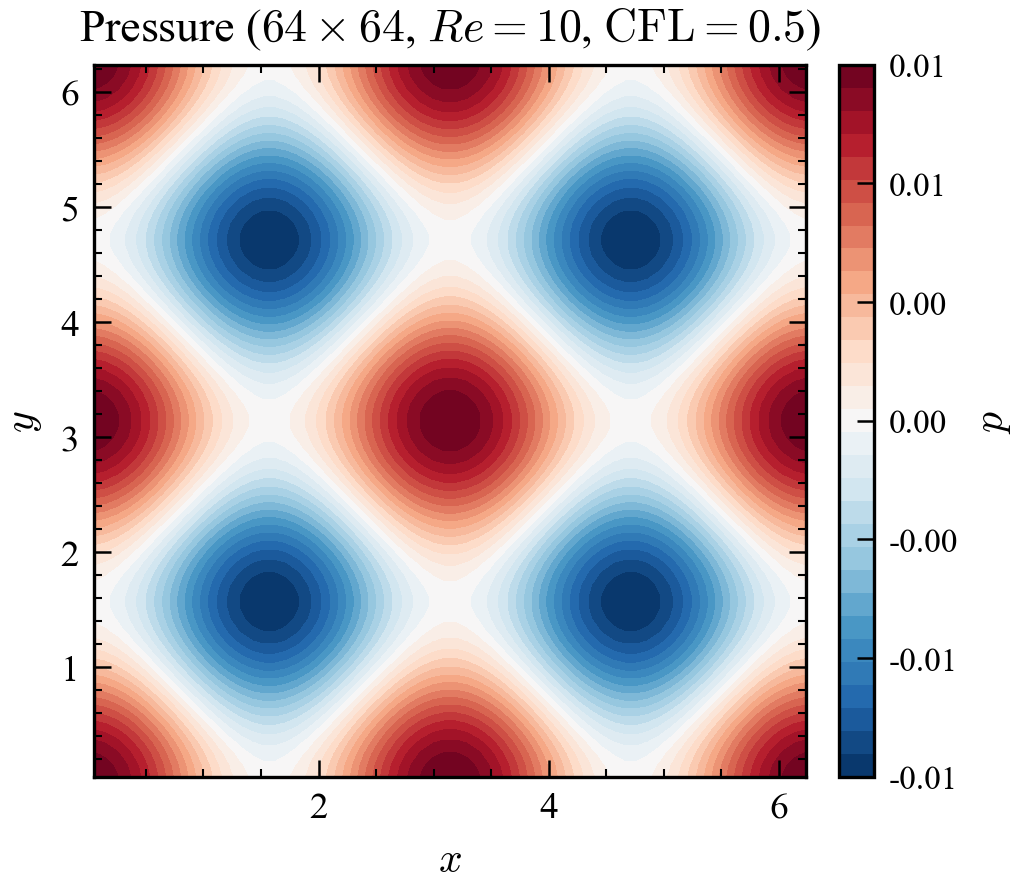
\includegraphics[width=0.32\textwidth]{images/pressure_re10_cfl0.5.png}
  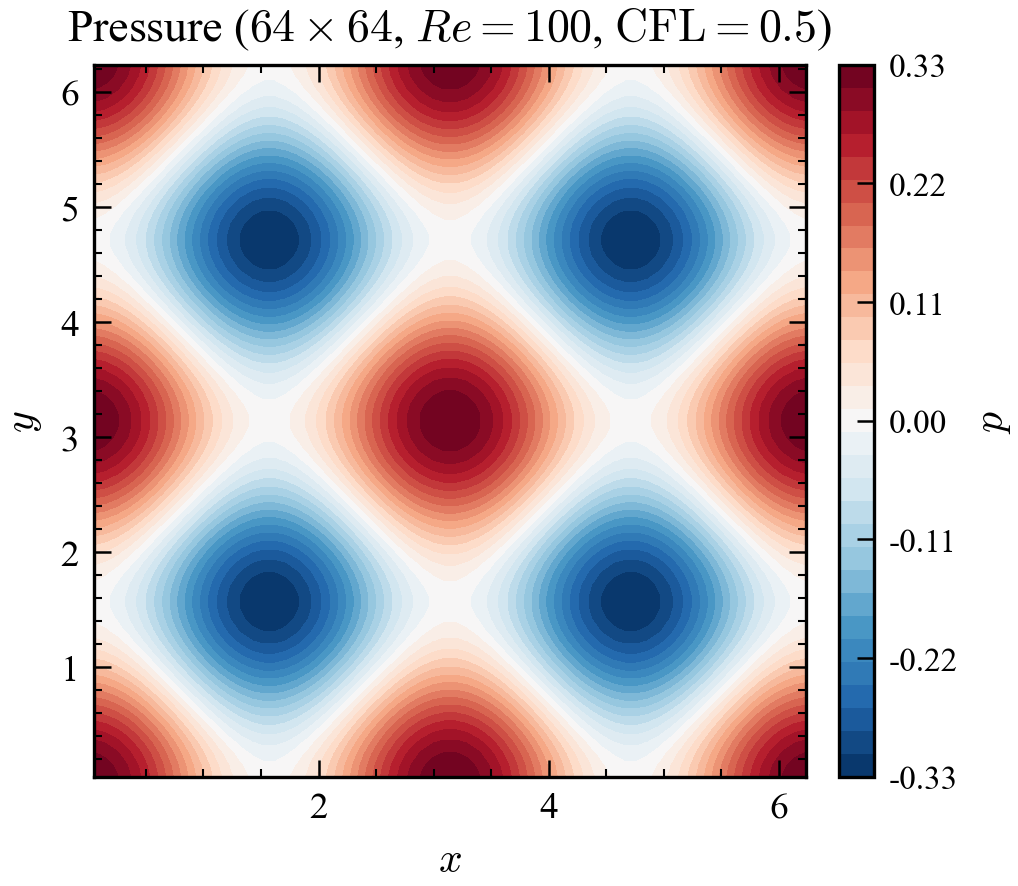
\includegraphics[width=0.32\textwidth]{images/pressure_re100_cfl0.5.png}
  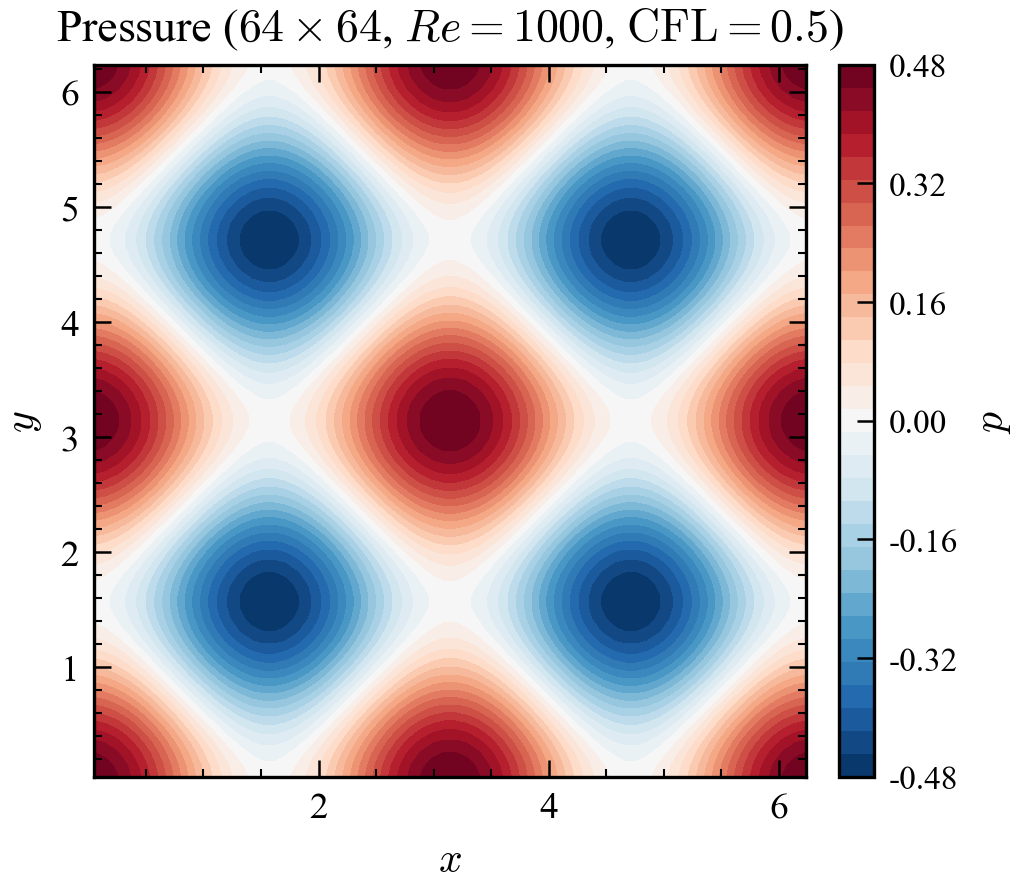
\includegraphics[width=0.32\textwidth]{images/pressure_re1000_cfl0.5.png}
  \caption{Pressure contours at $t=10$ on a $64\times64$ grid, $\mathrm{CFL} = 0.5$, for $\mathrm{Re} = 10$, $100$, and $1000$ (left to right). The four-fold pressure pattern reflects the two-by-two vortex arrangement of the Taylor--Green initial condition; amplitude decays with Re.}
  \label{fig:pressure}
\end{figure}

\begin{figure}[htbp]
  \centering
  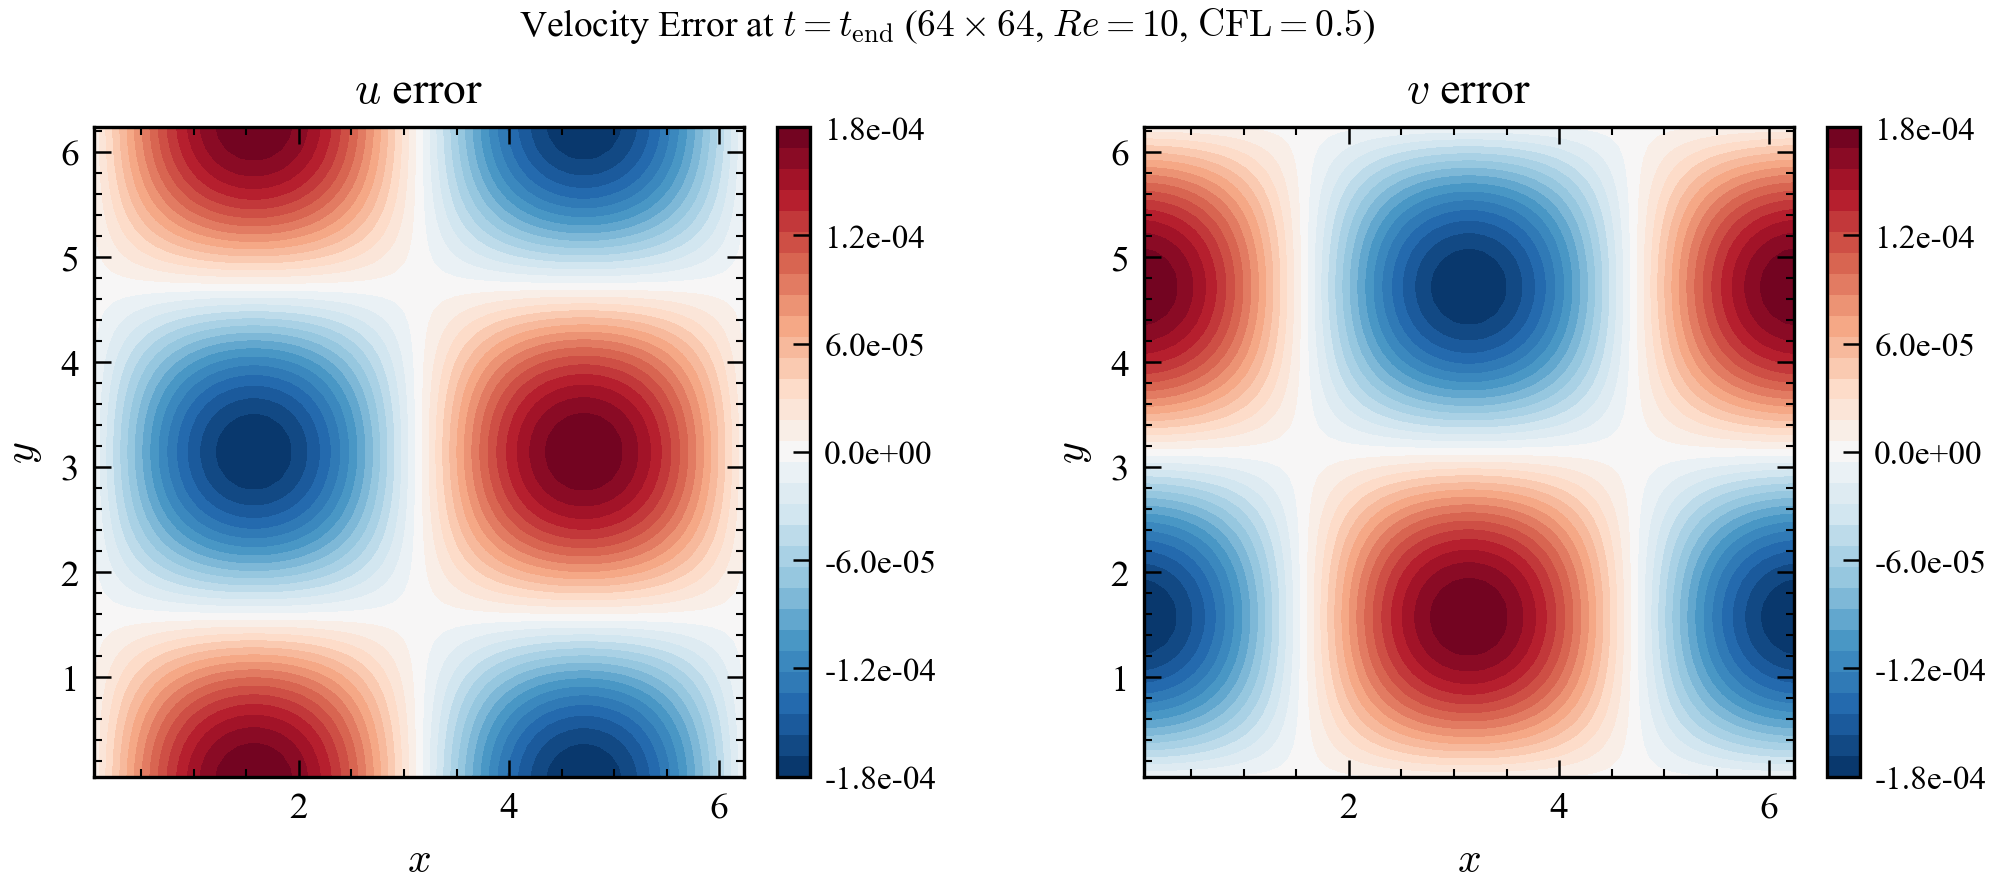
\includegraphics[width=0.6\textwidth]{images/velocity_error_re10_cfl0.5.png}\\[0.5em]
  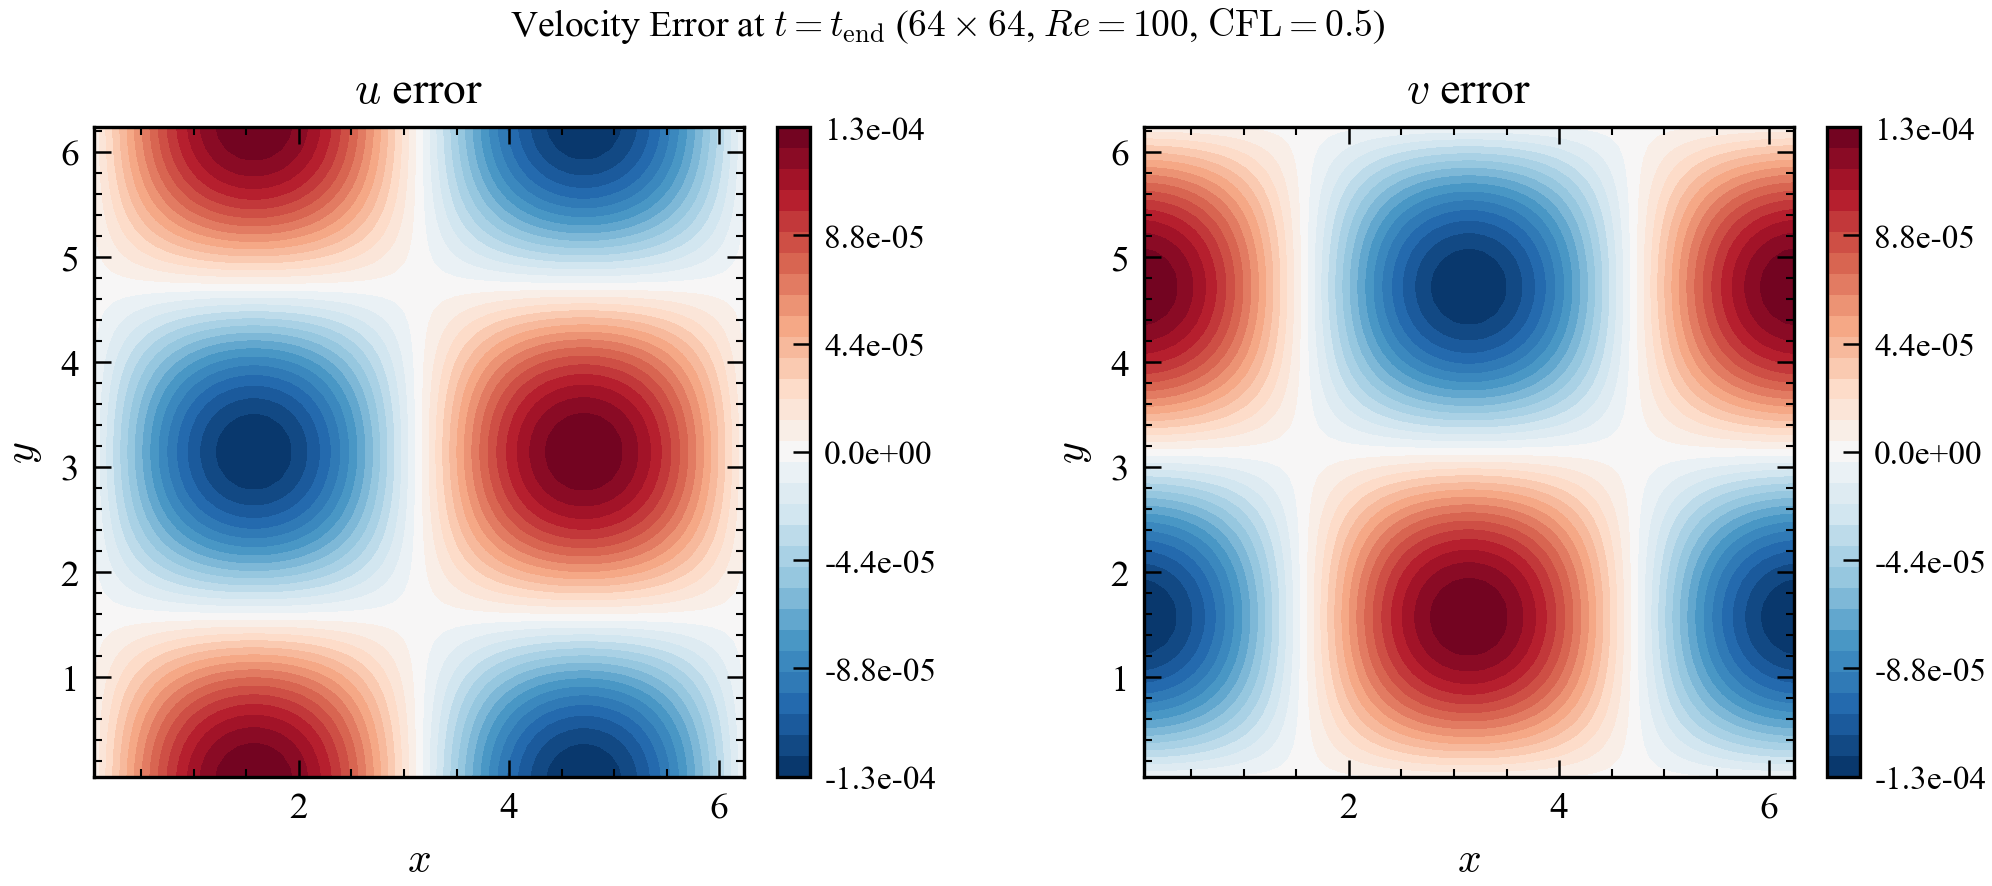
\includegraphics[width=0.6\textwidth]{images/velocity_error_re100_cfl0.5.png}\\[0.5em]
  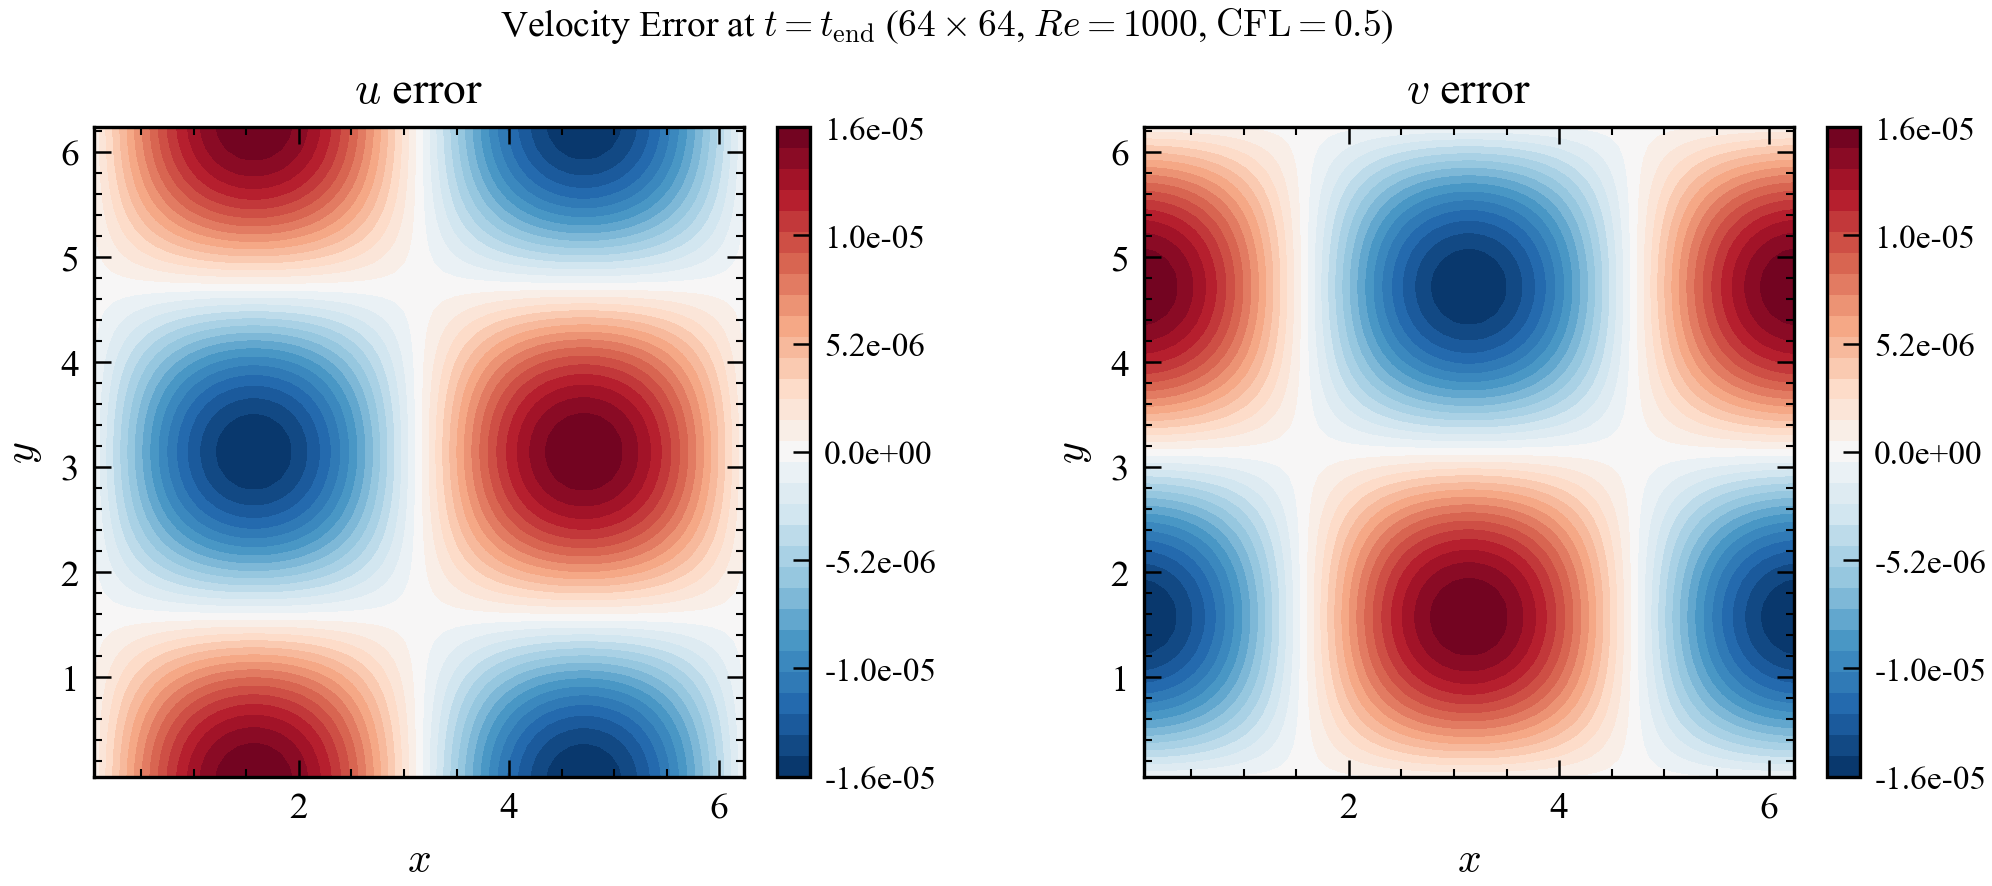
\includegraphics[width=0.6\textwidth]{images/velocity_error_re1000_cfl0.5.png}
  \caption{Velocity error $\|\mathbf{u} - \mathbf{u}_{\mathrm{exact}}\|_2$ vs.\ time on a $64\times64$ grid, $\mathrm{CFL} = 0.5$, for $\mathrm{Re} = 10$ (top), $100$ (middle), and $1000$ (bottom). The analytical Taylor--Green solution decays as $e^{-2t/\mathrm{Re}}$; error grows at higher Re where velocity magnitude is highest.}
  \label{fig:velocity_error}
\end{figure}


\subsubsection*{(e) Report}

% TODO: Report the following:
% - Time step size
% - Solver tolerances and number of iterations
% - Computational cost
% - Compare velocity field to analytical solution for 2D Taylor-Green vortex (see HW 1)

\begin{table}[htbp]
\centering
\caption{Solver performance summary for a $64\times 64$ grid at $\mathrm{CFL}=0.5$ and $t_{\mathrm{end}}=10$.}
\label{tab:solver_summary_cfl05}
\begin{tabular}{lccc}
\hline
Quantity & Re = 10 & Re = 100 & Re = 1000 \\
\hline
Grid & $64 \times 64$ & $64 \times 64$ & $64 \times 64$ \\
$t_{\mathrm{end}}$ & 10 & 10 & 10 \\
Steps & 90 & 185 & 202 \\
Wall time (s) & 3.7437 & 5.5666 & 4.5717 \\
Wall time/step (ms) & 41.5971 & 30.0897 & 22.6321 \\
\hline
$\Delta t_{\min}$ & 0.049147 & 0.049147 & 0.049147 \\
$\Delta t_{\mathrm{mean}}$ & 0.115126 & 0.054206 & 0.049638 \\
$\Delta t_{\max}$ & 0.362549 & 0.059980 & 0.050136 \\
\hline
RBGS iters min & 11 & 4 & 3 \\
RBGS iters mean & 20.31 & 4.00 & 3.00 \\
RBGS iters max & 53 & 4 & 3 \\
RBGS max residual & $9.98\times 10^{-9}$ & $2.12\times 10^{-9}$ & $2.47\times 10^{-12}$ \\
\hline
MG v-cycles min & 4 & 4 & 3 \\
MG v-cycles mean & 4.01 & 4.01 & 3.01 \\
MG v-cycles max & 5 & 5 & 5 \\
MG max residual & $6.77\times 10^{-9}$ & $6.83\times 10^{-9}$ & $6.84\times 10^{-9}$ \\
\hline
\end{tabular}
\end{table}


\subsubsection*{(f) Code}

See attached source code in the appendix.
